%________________________________________
%CaRS Move I “Establish a territory” (Situation):
% * Important area
% * Introducing and reviewing items of previous  research <--(ToDO)
Ship dynamics predictive models have a wide range of applications, e.g., safety enhancements, and route planning and optimization, autonomous shipping \citep{aslam_internet_2020}.
Ship manoeuvring is a sub-field of ship dynamics with well-established system-based models such as \citet{abkowitz_ship_1964,nomoto_steering_1957,norrbin_theory_1971}, and the MMG (manoeuvring modeling group) model \citep{yasukawa_introduction_2015}.

The captive model test is the classical method to identify the parameters within these models. However, for full-scale ships, this method is not practical. Computational fluid dynamics (CFD) with either unsteady Reynolds averaged Navier--Stokes (URANS) or steady Reynolds averaged Navier--Stokes (RANS) computations in virtual captive tests (VCTs) has emerged as an interesting option \citep{liu_predictions_2018,li_ship_2022}.
CFD requires a complete understanding of the system, which is straightforward for some simplified scenarios, but large modeling uncertainties from wind, wave, and current are expected when applied in a complex sea environment \citep{miller_ship_2021}. 
Even if the sea is flawlessly modeled, long-term predictions with high accuracy are exposed to deterministic chaos \citep{lorenz_deterministic_1963}.
With the other drawbacks of CFD in manoeuvring---such as high computational costs---data-driven models have become an attractive alternative or complement, with an increased number of publications in the past 10--15 years, %(shown in Fig.\ref{fig:pub_overview})
especially within the field of autonomous ships \citep{ahmed_survey_2023}, where predicting  ship trajectories is critical to avoid collisions. 

%Relevant paper keywords and their connections to the most recent research activities related to ship maneuvering modeling are presented in \autoref{fig:pub_overview}, where the circle size indicates how often the keywords occurred in the research articles. These papers claim their proposed regression-based methods can estimate the hydrodynamic coefficients of a ship’s maneuvering system accurately. However, most of the regression methods assume the exact “physical” model is known, i.e., the regression is based on “simulation” data, as indicated in \autoref{fig:pub_overview}, where the large circles of “simulation” and “maneuvering simulation” are directly connected with others.
%Most of the simulations (as shown in the keywords) were based on the model in \citet{fossen_handbook_2021}, such as the Gaussian process regression method in \citet{xue_system_2020} and the support vector machine method in \citet{wang_identification_2019} and \citet{wang_parameter_2021}. Recently, the support vector machine and neural network methods have also been used to identify the parameters of ship dynamic models using data from benchmark model tests with well-known ship maneuverability (e.g., SIMMAN, SHOPERA), as in \citet{wang_kernel-based_2020} and \citet{wakita_neural_2021}. The identified maneuvering models were validated by comparing their capabilities for trajectory prediction with either simulated or well-controlled model test results. However, the model accuracies in describing the ship’s kinetics, e.g., various forces acting on ships, was rarely mentioned. Nevertheless, such dynamic performance is essential to determine model feasibility for the application of a ship’s operation in real sea environments, i.e., with drifting caused by wind and current.
%%
%\begin{figure}[h]
%  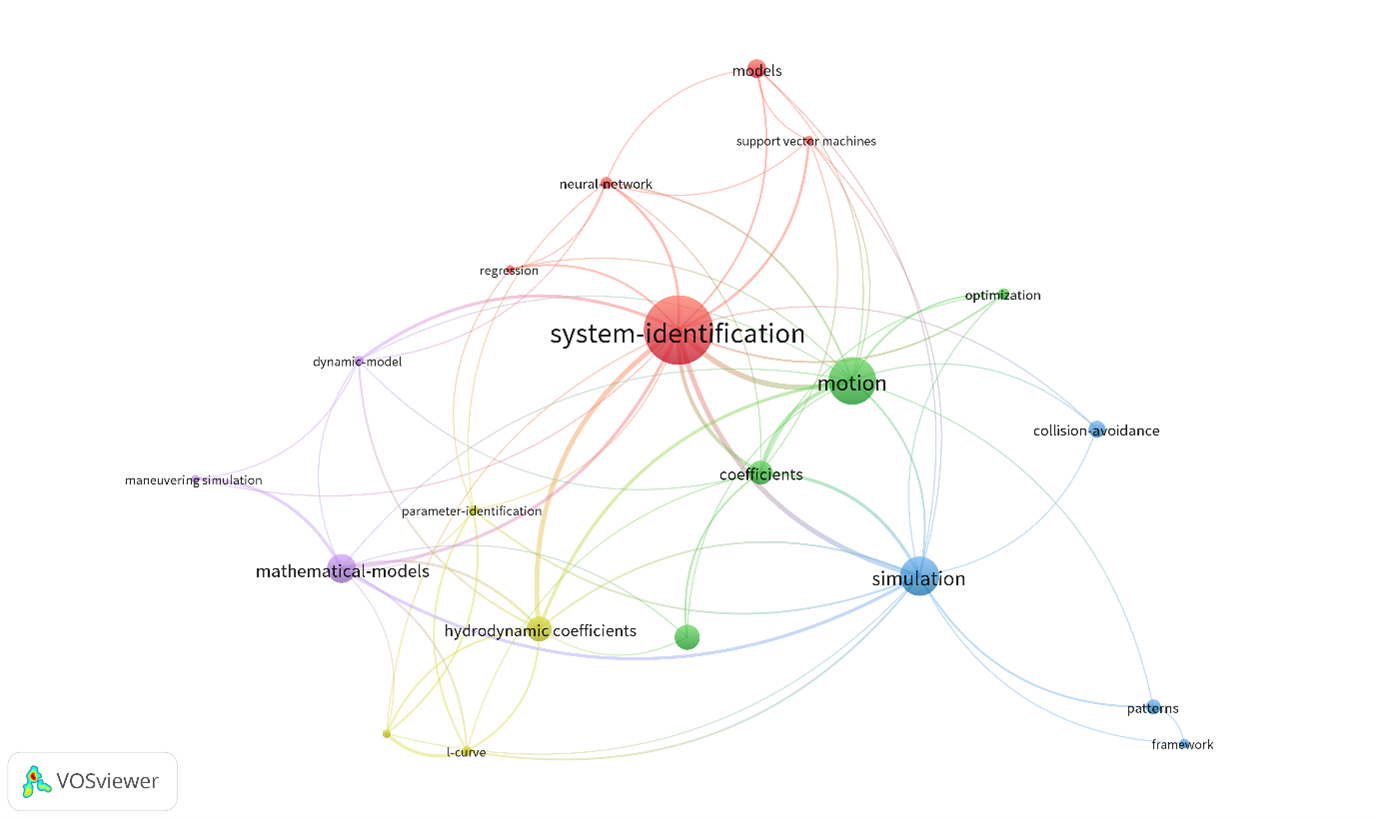
\includegraphics[width=\textwidth]{figures/keywords.png}
%  \caption{Research topics within the field of ship maneuverability system identification.}
%  \label{fig:pub_overview}
%\end{figure}
%%
%fication_1976} to develop a linear manoeuvring model that utilized manually recorded data in 1969 aboard the Atlantic Song freighter with Kalman filter (KF) and maximum likelihood estimation. 
%a_system_2015}, a 3 degree of freedom model by \citet{shi_identification_2009}, and a recursive EKF by \citet{alexandersson_system_2022}.
%KF for handling nonlinear systems, was used in \citet{revestido_herrero_two-step_2012}.
%\citet{zhu_parameter_2017}, and \citet{wang_parameter_2021}. 

%
%________________________________________
%CaRS Move II “Establish a niche” (Problem):
% * counter claim?
% * gap?
% * question       <------
% * continuation?
The regressors of the data-driven ship manoeuvring models are often strongly linearly dependent. 
In the beginning of a turning manoeuvre, side forces are primarily generated by the rudder; But very soon after, the ship will also have a yaw rate and drift angle, so that forces are also generated at the hull surface. The total force acting on the ship is normally used as the dependent variable in the regression, especially when the force from the rudder cannot be measured or estimated. The dependent variable is thus the sum of hull and rudder force, so that hull and rudder coefficients become strongly linearly dependent in the manoeuvre regression.
This multicollinearity is a well-known issue in parameter identification that may lead to parameter drift and poor generalization. The parameters are thus mathematically correct but physically incorrect \citep{luo_parameter_2016-1}. 
Using more informative data is perhaps the best way to mitigating the multicollinearity. When that is not feasible, simplifying the model is another commonly researched approach. 
Other possible remedies are the difference method \citep{luo_parameter_2016-1}, principal component analysis (PCA), and partial least-squares regression \citep{jian-chuan_parametric_2015}.
%________________________________________
%CaRS Move III “Occupy the niche” (Solution/Evaluation):
% * outline purpose?                        <--
% * list research questions?                <--
% * announce principal findings?            
% * stating the value of present research?
% * article structure?                      <--

Other remedies are however needed. Therefore, a physics-informed manoeuvring model (PI model) is proposed in the present paper, which features a new semi-empirical rudder model to estimate the rudder forces. The rudder and hull forces are then separated in the regression, to reduce the multicollinearity. The PI model is compared to a more conventional physics uninformed model (PU model) with respect to: 
\begin{itemize}
    \item Parameter drift.
    \item Generalization.
    \item The physical correctness of the identified models.
\end{itemize}
The parameter drift is studied in a sensitivity analysis. The generalization is studied by exposing a model identified on calm water zigzag tests to wind, which is a state where the ship has a drift angle but no yaw rate. The zigzag test contains little information about this state, as shown in the phase portrait in \autoref{fig:phase_portrait}. There are in fact only six points where the yaw rate is zero, where the phase portrait crosses the x-axis. 
%This drifting (side forces) is rarely investigated as shown in %\autoref{fig:pub_overview}.
\begin{figure}[h]
  \centering
  \includesvg{figures/multicollineraity.multicollinearity.svg}
  \caption{Phase portrait where the combination of drift angle and yaw rate is shown for zigzag10/10 and zigzag20/20 wPCC model tests.}
  \label{fig:phase_portrait}
\end{figure}

The physical correctness of the identified PI and PU models is assessed by comparison with a reference model. The reference model is established from virtual captive tests (VCT) based on CFD calculations. The model is assumed to resemble the true hydrodynamics.  

A wind-powered pure car carrier (wPCC) is the main test case in the present paper. 
This ship has much larger rudders than conventional ships---to improve the sailing performance---
which increases the demand for physically correct rudder modeling.

A brief description of the workflow of this research is shown in \autoref{fig:methodology}.
The PI and PU models are identified on free sailing model tests \citep{alexandersson_system_2022,alexandersson_wpcc_2024} via inverse dynamics (ID) and regression. To assess the physical correctness, a reference model is established, where the PI model is instead identified on a VCT dataset. This reference model, based on CFD, is assumed to be a sufficiently correct representation of the ship's physics.
Verification and comparisons between the models are carried out on the free sailing model tests.
%
\begin{figure}[h]
  \centering
  %\includesvg[width=\columnwidth, pretex=\scriptsize, height=12cm]{figures/methodology2.svg}
  \includesvg[pretex=\centering\fontsize{7.5}{8}]{figures/methodology2.svg}
  \caption{Research workflow, describing how the reference model was obtained }
  \label{fig:methodology}
\end{figure}

The remainder of this paper is organized as follows: The proposed PI model is first presented together with the PU 
 model in \autoref{sec:ship_models}, while mathematical details of the models are given in the appendix. 
\autoref{sec:methodology} describes the developed methodology framework to identify parameters within the PI model, including VCT-- and ID--regressions. The case study ship is briefly described in \autoref{sec:case_study}, along with known parameters of the ship’s manoeuvring model. \autoref{sec:results} provides the results for the wPCC. Results for the KVLCC2 test case are also presented, followed by key conclusions of this research in \autoref{sec:conclusions}.